%=============================================================================
% SECTION 2: MATHEMATICAL FORMALISM
% DFD Unified Review --- Part I: Foundations
%=============================================================================

\section{Mathematical Formalism}\label{sec:formalism}

This section develops the complete mathematical structure of Density Field 
Dynamics: the optical metric governing light propagation, the action principle, 
field equations, and the family of crossover functions. The presentation aims 
for both rigor and physical transparency.

%-----------------------------------------------------------------------------
% §2.1 THE OPTICAL METRIC AND KINEMATICS
%-----------------------------------------------------------------------------
\subsection{The Optical Metric and Geodesics}\label{sec:optical_metric}

\subsubsection{Gordon's Optical Metric}

The optical metric approach has a distinguished history in relativity and 
optics. Gordon~\cite{Gordon1923} showed in 1923 that electromagnetic waves 
propagating through a moving dielectric medium experience an effective 
spacetime geometry. Perlick~\cite{Perlick2000} systematically developed 
ray optics in curved spacetimes, establishing the mathematical foundations 
for relating wave propagation to null geodesics.

\DFD adopts this framework but makes a conceptual inversion: rather than 
deriving an effective optical metric from an underlying curved spacetime, 
the optical refractive index becomes the fundamental gravitational degree 
of freedom on flat Minkowski spacetime.

The optical metric is defined by the single scalar field $\psifield(\mathbf{x}, t)$:
\begin{equation}
d\tilde{s}^2 = -\frac{c^2\,dt^2}{n^2(\mathbf{x},t)} + d\mathbf{x}^2, 
\qquad n(\mathbf{x},t) = e^{\psifield(\mathbf{x},t)}.
\label{eq:optical_metric_full}
\end{equation}
The line element $d\tilde{s}^2 = 0$ defines null rays---the trajectories 
of light. The refractive index $n = e^\psi$ satisfies $n > 0$ everywhere, 
ensuring light propagation is always well-defined.

\subsubsection{Fermat's Principle}

Light rays extremize optical path length. For a path $\mathbf{x}(s)$ 
parameterized by arc length:
\begin{equation}
\delta \int n(\mathbf{x})\,ds = 0.
\label{eq:fermat}
\end{equation}
The Euler-Lagrange equations yield the ray equation:
\begin{equation}
\frac{d}{ds}\left(n\frac{d\mathbf{x}}{ds}\right) = \nabla n,
\end{equation}
which governs the bending of light in the refractive medium. For small 
deflections, this reproduces Snell's law in differential form.

The connection to null geodesics is established by noting that the 
optical metric~\eqref{eq:optical_metric_full} is a diagonal metric 
with position-dependent lapse $c/n$; its null geodesics coincide 
with extremals of Fermat's principle.

\subsubsection{Phase and Group Velocities}

The one-way phase velocity is
\begin{equation}
c_{\rm phase} = \frac{c}{n} = c\,e^{-\psi}.
\end{equation}
In a gravitational potential well ($\psi > 0$), light slows: $c_{\rm phase} < c$. 
The coordinate speed of light depends on position, but the two-way 
speed---measured by local clocks and rods---remains $c$.

For the group velocity in the nondispersive band (where $dn/d\omega = 0$), 
group and phase velocities coincide: $c_{\rm group} = c_{\rm phase}$.

\paragraph{Note on asymptotic propagation.}
This effective-medium (optical metric) description does not imply an 
asymptotic EM--GW speed split. The GW170817 constraint 
$|c_T/c - 1| < 10^{-15}$ is satisfied because (i)~the TT sector has 
no derivative mixing with $\psi$ in its principal part 
(\S\ref{sec:gw-twosector}), and (ii)~the leading propagation delay 
is common-mode when EM and GW arrivals are compared using receiver clocks.

%-----------------------------------------------------------------------------
% §2.2 ACTION PRINCIPLE
%-----------------------------------------------------------------------------
\subsection{Action Principle}\label{sec:action}

\subsubsection{Scalar Sector Action}

The scalar field $\psifield$ is governed by a k-essence-type action with 
a nonlinear kinetic term:
\begin{equation}
S_\psi = \int dt\,d^3x \left\{ 
  \frac{\astar^2}{8\pi G}\,\Wfunc\!\left(\frac{|\nabla\psifield|^2}{\astar^2}\right) 
  - \frac{c^2}{2}\psifield(\rho - \bar{\rho}) 
\right\},
\label{eq:action_scalar}
\end{equation}
where:
\begin{itemize}
\item $\Wfunc(y)$ is a dimensionless potential with $\Wfunc(0) = 0$, 
$\Wfunc'(0) = 1$, and convexity $\Wfunc''(y) \geq 0$.
\item $\astar$ is the characteristic gradient scale with $[\astar] = 1/\text{m}$. 
It relates to the MOND acceleration scale $a_0 = 2\sqrt{\alpha}\,cH_0 \approx 1.2 \times 10^{-10}\,\si{m/s^2}$ via 
$\astar = 2a_0/c^2$. The argument $y = |\nabla\psi|^2/\astar^2$ is then dimensionless.
\item $\rho$ is the local mass density; $\bar{\rho}$ is the mean cosmic 
density, ensuring proper cosmological boundary conditions.
\end{itemize}

The kinetic function $\Wfunc(|\nabla\psi|^2/\astar^2)$ interpolates between:
\begin{itemize}
\item \textbf{High gradients} ($|\nabla\psi|/\astar \gg 1$): 
$\Wfunc \approx y$, yielding linear (Newtonian) behavior.
\item \textbf{Low gradients} ($|\nabla\psi|/\astar \ll 1$): 
$\Wfunc \sim \sqrt{y}$, producing MOND-like deep-field dynamics.
\end{itemize}

\paragraph{Dimensional verification.}
Note: In the Lagrangian, $\astar$ has units of $1/\text{m}$ (a gradient scale), 
related to the physical acceleration scale $a_0$ by $\astar = 2a_0/c^2$. This ensures 
$|\nabla\psi|/\astar$ is dimensionless. Substituting $\astar = 2a_0/c^2$ into 
$\astar^2/(8\pi G)$ yields a factor with correct energy-density dimensions.
The matter coupling $c^2\psi\rho$ has units:
\begin{itemize}
\item $[c^2\psi\rho]$ = $(\text{m/s})^2 \cdot 1 \cdot (\text{kg/m}^3)$ 
= $\text{kg}/(\text{m}\cdot\text{s}^2)$ (energy density)
\end{itemize}
Both terms integrate to energy $\times$ time: $[S_\psi]$ = J$\cdot$s $\checkmark$

\paragraph{Comparison with AQUAL.}
The action~\eqref{eq:action_scalar} is the scalar-field analogue of 
Bekenstein-Milgrom's AQUAL formulation~\cite{BekensteinMilgrom1984}. 
The key differences are: (i)~the fundamental field is $\psi$ (determining 
refractive index $n = e^\psi$) rather than the potential $\Phi$ directly; 
(ii)~the coupling to matter goes through the optical metric, not just the 
potential; (iii)~the $\mu$-crossover is constrained by optical consistency 
(positive $n$, well-posed wave propagation).

\paragraph{Status of Eq.~\eqref{eq:action_scalar}.}
Equation~\eqref{eq:action_scalar} is the \emph{quasi-static spatial sector} used for lensing, weak-field dynamics, and galactic phenomenology.  The temporal completion is derived separately in Appendix~\ref{app:temporal-completion}, where the unique local temporal invariant $\Delta \equiv (c/a_0)|\dot\psi - \dot\psi_0|$ is introduced and the dust branch $w\to 0$, $c_s^2\to 0$ is proved.  The full scalar-sector action combining spatial and temporal sectors is
\begin{align}\label{eq:action-full-dynamic}
S_\psi = \int dt\,d^3x\;\Biggl\{
  &\frac{a_*^2}{8\pi G}\biggl[
    W\!\biggl(\frac{|\nabla\psi|^2}{a_*^2}\biggr)
    + K\!\biggl(\frac{c}{a_0}|\dot\psi{-}\dot\psi_0|\biggr)
  \biggr] \notag\\
  &- \frac{c^2}{2}\,\psi(\rho - \bar\rho)
\Biggr\}.
\end{align}
where $K$ is the temporal kinetic function with $K'(\Delta) = \mu(\Delta)$.

\paragraph{Convexity and stability.}
The function $\Wfunc$ must be convex ($\Wfunc'' \geq 0$) to ensure:
\begin{enumerate}
\item Positive-definite energy density
\item Well-posed elliptic field equations
\item No ghost instabilities
\end{enumerate}
This follows from standard variational theory: a convex energy functional 
has a unique minimizer, and small perturbations about the minimum have 
positive energy.

%-----------------------------------------------------------------------------
\subsubsection{Matter Coupling}

Matter couples to the physical metric $\tilde{g}_{\mu\nu}$:
\begin{equation}\label{eq:physical-metric}
\tilde{g}_{\mu\nu} = \text{diag}\!\left(-c^2 e^{-\psi},\; e^{+\psi},\; e^{+\psi},\; e^{+\psi}\right).
\end{equation}
This shares the same null cone as the Gordon eikonal 
metric~\eqref{eq:optical_metric_full}: setting $d\tilde{s}^2 = 0$ gives 
$|d\mathbf{x}/dt| = c\,e^{-\psi} = c/n$, so light propagation is 
identical. The exponential structure $n = e^\psi$ uniquely fixes the 
relation between time and spatial components (cf.\ the PPN 
derivation in \S\ref{sec:ppn-gamma-beta}).
For a point particle of mass $m$, the action is:
\begin{equation}
S_{\rm pp} = -mc \int d\tau\,\sqrt{-\tilde{g}_{\mu\nu}\frac{dx^\mu}{d\tau}\frac{dx^\nu}{d\tau}}.
\end{equation}
In the non-relativistic limit ($v \ll c$, $|\psi| \ll 1$):
\begin{equation}
S_{\rm pp} \approx -mc^2 \int dt\left(1 - \frac{v^2}{2c^2} - \frac{\Phipot}{c^2}\right),
\label{eq:pp_action}
\end{equation}
where $\Phipot = -c^2\psi/2$ is the effective Newtonian potential. 
The equation of motion is:
\begin{equation}
\frac{d^2\mathbf{x}}{dt^2} = -\nabla\Phipot = \frac{c^2}{2}\nabla\psi = \avec,
\end{equation}
confirming that all test masses fall with acceleration 
$\avec = (c^2/2)\nabla\psi$---the Weak Equivalence Principle is satisfied.

%-----------------------------------------------------------------------------
\subsubsection{Gravitational Wave Sector}

The transverse-traceless (TT) gravitational wave sector is embedded with 
the standard linearized action:
\begin{equation}
S_h = \frac{c^4}{32\pi G}\int dt\,d^3x \left[
  \frac{1}{c^2}(\partial_t h_{ij}^{\rm TT})^2 - (\nabla h_{ij}^{\rm TT})^2
\right].
\label{eq:action_gw}
\end{equation}
This is the canonical form for a massless spin-2 field on flat spacetime, 
ensuring:
\begin{itemize}
\item Propagation speed $c_T = c$ (consistent with GW170817)
\item Two tensor polarizations ($+$ and $\times$)
\item No scalar or vector GW modes
\end{itemize}
The wave equation follows from variation:
\begin{equation}
\Box h_{ij}^{\rm TT} = -\frac{16\pi G}{c^4}(T_{ij}^{\rm eff})^{\rm TT},
\label{eq:wave_equation}
\end{equation}
where $\Box = c^{-2}\partial_t^2 - \nabla^2$ and $(T_{ij}^{\rm eff})^{\rm TT}$ 
is the transverse-traceless projection of the effective stress-energy tensor.

%-----------------------------------------------------------------------------
\subsubsection{Interaction and Complete Action}

The gravitational wave sector couples to matter through:
\begin{equation}
S_{\rm int} = -\frac{1}{2}\int d^4x\,h_{ij}^{\rm TT} T^{ij}_{\rm eff},
\end{equation}
with the effective stress-energy tensor:
\begin{equation}
T^{ij}_{\rm eff} = \rho v^i v^j + p\delta^{ij} + \order{v^4/c^4}.
\end{equation}

The complete \DFD action is:
\begin{equation}
\boxed{
S_{\rm DFD} = S_\psi + S_h + S_{\rm int} + S_{\rm matter}
}
\label{eq:complete_action}
\end{equation}
where $S_{\rm matter}$ includes all matter field Lagrangians minimally 
coupled to the optical metric.

\begin{table}[t]
\caption{Action sectors and their physical content.}
\label{tab:action_sectors}
\begin{ruledtabular}
\begin{tabular}{lll}
Sector & Content & Degrees of Freedom \\
\hline
$S_\psi$ & Scalar refractive field & 1 (scalar $\psi$) \\
$S_h$ & TT gravitational waves & 2 (tensor $h_{ij}^{\rm TT}$) \\
$S_{\rm int}$ & GW-matter coupling & --- \\
$S_{\rm matter}$ & Matter fields & Various \\
\end{tabular}
\end{ruledtabular}
\end{table}

\paragraph{Key properties of the complete action:}
\begin{itemize}
\item \textbf{Explicit variational principle:} All field equations derivable 
from $\delta S = 0$.
\item \textbf{Energy positivity:} $\Wfunc$ convex ensures no negative-energy modes.
\item \textbf{No ghosts:} Single scalar DOF in $\psi$; two tensor DOFs in $h_{ij}^{\rm TT}$.
\item \textbf{GW speed $c_T = c$:} Built into the TT action.
\item \textbf{Newtonian limit:} $\mu \to 1$ for large $|\nabla\psi|/\astar$.
\item \textbf{MOND limit:} $\mu \sim x$ for small $|\nabla\psi|/\astar$.
\end{itemize}

%-----------------------------------------------------------------------------
% §2.3 FIELD EQUATIONS
%-----------------------------------------------------------------------------
\subsection{Field Equations}\label{sec:field_equations}

\subsubsection{General Nonlinear Form}

Variation of $S_\psi$ with respect to $\psi$ yields the fundamental 
field equation:
\begin{equation}
\nabla \cdot \left[\mufunction\!\left(\frac{|\nabla\psifield|}{\astar}\right)
\nabla\psifield\right] = -\frac{8\pi G}{c^2}(\rho - \bar{\rho}),
\label{eq:field_general}
\end{equation}
where the response function $\mufunction(x)$ is related to the kinetic 
potential by:
\begin{equation}
\mufunction(x) = \Wfunc'(x^2) + 2x^2\Wfunc''(x^2), \qquad x = \frac{|\nabla\psi|}{\astar}.
\end{equation}

\paragraph{Derivation sketch.}
From action~\eqref{eq:action_scalar}, compute:
\begin{align}
\frac{\delta S_\psi}{\delta\psi} &= -\frac{\astar^2}{8\pi G}\nabla\cdot
\left[\Wfunc'\!\left(\frac{|\nabla\psi|^2}{\astar^2}\right)
\frac{2\nabla\psi}{\astar^2}\right] - \frac{c^2}{2}(\rho - \bar{\rho}) \nonumber\\
&= -\frac{1}{4\pi G}\nabla\cdot\left[\Wfunc'(X)\nabla\psi\right] 
- \frac{c^2}{2}(\rho - \bar{\rho}),
\end{align}
where $X = |\nabla\psi|^2/\astar^2$. Setting $\delta S/\delta\psi = 0$ and 
identifying $\mu(x) = \Wfunc'(x^2)$ (for the simple case) gives 
Eq.~\eqref{eq:field_general}.

%-----------------------------------------------------------------------------
\subsubsection{Acceleration Form with $a^2$ Invariant}

An illuminating alternative form uses the physical acceleration field 
$\avec = (c^2/2)\nabla\psi$. Defining the acceleration-squared invariant 
$\asq \equiv \avec \cdot \avec$, we have:
\begin{equation}
|\nabla\psi|^2 = \frac{4\asq}{c^4}.
\end{equation}
Substituting into Eq.~\eqref{eq:field_general} and simplifying yields 
the master equation:
\begin{equation}
\boxed{
\nabla \cdot \avec + \frac{\ka}{c^2}\asq = -4\pi G\rho
}
\label{eq:master_acceleration}
\end{equation}
where $\ka$ is a dimensionless self-coupling constant. 
In \DFD, the $\alpha$-relation (\S\ref{sec:alpha}) predicts:
\begin{equation}
\ka = \frac{3}{8\alphafine} \approx 51.4.
\end{equation}

\paragraph{Dimensional consistency.}
All three terms in Eq.~\eqref{eq:master_acceleration} have dimensions 
of inverse time squared:
\begin{itemize}
\item $[\nabla \cdot \avec] = (\text{m/s}^2)/\text{m} = \text{s}^{-2}$
\item $[\ka\asq/c^2] = 1 \cdot (\text{m/s}^2)^2/(\text{m/s})^2 = \text{s}^{-2}$
\item $[4\pi G\rho] = (\text{m}^3/\text{kg}\cdot\text{s}^2)(\text{kg/m}^3) = \text{s}^{-2}$
\end{itemize}

%-----------------------------------------------------------------------------
\subsubsection{Regime Hierarchy}

Comparing the divergence and self-interaction terms in 
Eq.~\eqref{eq:master_acceleration} reveals three regimes:

\begin{table}[h]
\caption{Regime hierarchy in DFD.}
\label{tab:regimes}
\begin{ruledtabular}
\begin{tabular}{lll}
Regime & Condition & Behavior \\
\hline
Solar/high-$a$ & $\nabla\cdot\avec \gg \ka\asq/c^2$ & 
  Newtonian (GR limit) \\
Crossover & $\nabla\cdot\avec \sim \ka\asq/c^2$ & 
  MOND-like transition \\
Deep-field/low-$a$ & $\nabla\cdot\avec \ll \ka\asq/c^2$ & 
  Nonlinear $\asq \propto a_N$ \\
\end{tabular}
\end{ruledtabular}
\end{table}

In the Solar System ($a \sim 10^{-3}\,\text{m/s}^2$), the self-interaction 
is negligible: $\ka\asq/c^2 \sim 10^{-19}\,\text{s}^{-2}$, whereas 
$\nabla\cdot\avec \sim 10^{-6}\,\text{s}^{-2}$. The theory reduces to 
standard Newtonian gravity (and, with relativistic corrections, to GR).

In galactic outskirts ($a \sim 10^{-10}\,\text{m/s}^2$), both terms 
are comparable, and the nonlinear $\mu$-crossover becomes important. 
This is the regime where MOND-like phenomenology emerges.

% FIGURE 3: Regime diagram (placeholder)
\begin{figure}[t]
\centering
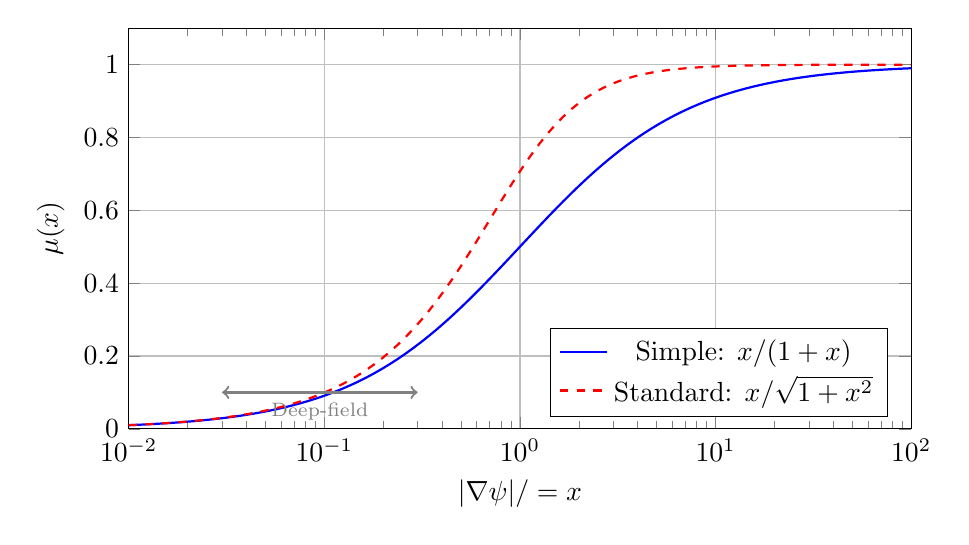
\begin{tikzpicture}
\begin{semilogxaxis}[
  width=0.95\columnwidth,
  height=0.55\columnwidth,
  xlabel={$|\nabla\psi|/\astar = x$},
  ylabel={$\mu(x)$},
  xmin=0.01, xmax=100,
  ymin=0, ymax=1.1,
  legend pos=south east,
  grid=major
]
% Simple $\mu$
\addplot[thick, blue, domain=0.01:100, samples=100] {x/(1+x)};
\addlegendentry{Simple: $x/(1+x)$}
% Standard $\mu$
\addplot[thick, red, dashed, domain=0.01:100, samples=100] {x/sqrt(1+x^2)};
\addlegendentry{Standard: $x/\sqrt{1+x^2}$}
% Regime annotations
\draw[<->, thick, gray] (axis cs:0.03,0.1) -- (axis cs:0.3,0.1) 
  node[midway, below] {\scriptsize Deep-field};
\draw[<->, thick, gray] (axis cs:3,0.1) -- (axis cs:30,0.1) 
  node[midway, below] {\scriptsize Solar};
\end{semilogxaxis}
\end{tikzpicture}
\caption{The $\mu(x)$ crossover function interpolates between deep-field 
($\mu \sim x$) and solar ($\mu \to 1$) regimes. The transition occurs 
at $x \sim 1$, corresponding to $|\nabla\psi| \sim \astar$. The ``Standard'' form is shown for historical comparison; the $S^3$ microsector uniquely selects the ``Simple'' form (Appendix~\ref{app:mu-derivation}).}
\label{fig:regimes}
\end{figure}

%-----------------------------------------------------------------------------
% §2.4 THE $\mu$ CROSSOVER FUNCTION
%-----------------------------------------------------------------------------
\subsection{The $\mufunction(x)$ Crossover Function}\label{sec:mu_function}

The response function $\mufunction(x)$ must satisfy four physical constraints:

\begin{enumerate}
\item \textbf{Solar limit:} $\mufunction(x) \to 1$ as $x \to \infty$ 
(recover Poisson equation).
\item \textbf{Deep-field limit:} $\mufunction(x) \sim x$ as $x \to 0$ 
(MOND-like scaling for flat rotation curves).
\item \textbf{Monotonicity:} $\mufunction'(x) > 0$ for $x > 0$ 
(strict ellipticity of field equation).
\item \textbf{Convexity:} The associated $\Wfunc$ must be convex 
(energy positivity, stability).
\end{enumerate}

\subsubsection{Admissible Families}

Table~\ref{tab:mu_catalog} catalogs the $\mu$-functions used in the \DFD literature. The ``Simple'' form $\mu(x) = x/(1+x)$ is \textbf{uniquely derived} from the $S^3$ microsector via a composition law (Appendix~\ref{app:mu-derivation}, Theorem~\ref{thm:mu-theorem}).

\begin{table}[h]
\caption{Catalog of admissible $\mu(x)$ functions. The Simple form is derived from topology.}
\label{tab:mu_catalog}
\begin{ruledtabular}
\begin{tabular}{llcc}
Name & Formula & $\mu(1)$ & Status \\
\hline
Simple & $\displaystyle\frac{x}{1+x}$ & $1/2$ & \textbf{Derived} \\[8pt]
Standard & $\displaystyle\frac{x}{\sqrt{1+x^2}}$ & $1/\sqrt{2}$ & Phenomenological \\[8pt]
General & $\displaystyle\frac{x}{(1+\lambda x^\alpha)^{1/\alpha}}$ & varies & Phenomenological \\[8pt]
Exponential & $1 - e^{-x}$ & $1-e^{-1}$ & Phenomenological \\
\end{tabular}
\end{ruledtabular}
\end{table}

The two-parameter general family $\mu_{\alpha,\lambda}(x)$ is particularly 
useful for fitting EHT shadow data and ppE gravitational wave coefficients. 
It satisfies all four constraints for $\alpha \geq 1$ and $\lambda > 0$.

% FIGURE 2: $\mu$ family (adapted from Strong-GW)
\begin{figure}[t]
\centering
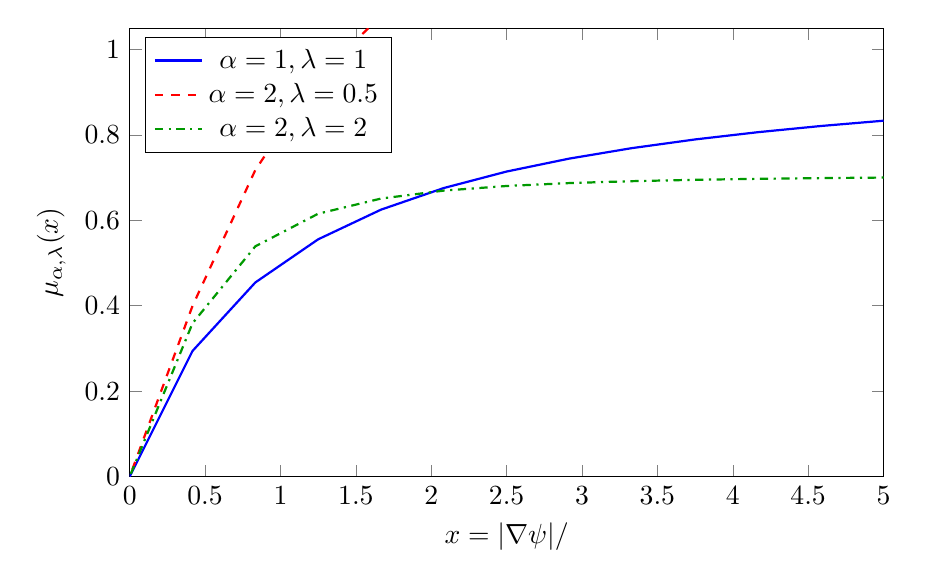
\begin{tikzpicture}
\begin{axis}[
  width=0.92\columnwidth,
  height=0.6\columnwidth,
  xlabel={$x = |\nabla\psi|/\astar$},
  ylabel={$\mu_{\alpha,\lambda}(x)$},
  xmin=0, xmax=5,
  ymin=0, ymax=1.05,
  legend style={at={(0.02,0.98)}, anchor=north west}
]
\addplot[thick, blue] {x/(1+x)^(1)};
\addlegendentry{$\alpha=1, \lambda=1$}
\addplot[thick, red, dashed] {x/(1+0.5*x^2)^(1/2)};
\addlegendentry{$\alpha=2, \lambda=0.5$}
\addplot[thick, green!60!black, dashdotted] {x/(1+2*x^2)^(1/2)};
\addlegendentry{$\alpha=2, \lambda=2$}
\end{axis}
\end{tikzpicture}
\caption{Constrained crossover functions $\mu_{\alpha,\lambda}(x)$: 
linear at small $x$ (deep-field), saturating at large $x$ (solar limit), 
monotone and convex throughout.}
\label{fig:mu_family}
\end{figure}

\subsubsection{Single Calibration Freeze}

The $\mu$-function parameters are calibrated \emph{once} on the baryonic 
Radial Acceleration Relation (RAR)~\cite{McGaugh2016RAR} and frozen for 
all other predictions. No retuning is performed for laboratory, lensing, 
GW, or strong-field applications. This converts the deep-field behavior 
from arbitrary curve-fitting to a single phenomenological calibration, 
analogous to fixing $\azero$ in MOND.

%-----------------------------------------------------------------------------
% §2.5 CONSERVED QUANTITIES
%-----------------------------------------------------------------------------
\subsection{Conserved Quantities and Symmetries}\label{sec:conservation}

\subsubsection{Diffeomorphism Invariance}

The action~\eqref{eq:complete_action} is invariant under spatial 
diffeomorphisms on the flat background. This generates a conserved 
stress-energy tensor in the optical metric:
\begin{equation}
\tilde{\nabla}_\mu \tilde{T}^{\mu\nu} = 0,
\end{equation}
where $\tilde{\nabla}$ is the covariant derivative with respect to 
$\tilde{g}_{\mu\nu}$.

\subsubsection{Energy Conservation}

In static configurations, the total energy functional:
\begin{equation}
E[\psi] = \int d^3x \left[\frac{\astar^2}{8\pi G}\Wfunc\!\left(
\frac{|\nabla\psi|^2}{\astar^2}\right) + \frac{c^2}{2}\rho\psi\right]
\end{equation}
is minimized by solutions of the field equation. The convexity of $\Wfunc$ 
ensures $E[\psi] \geq 0$ for all configurations satisfying appropriate 
boundary conditions.

\subsubsection{Local Conservation in PPN Framework}

Within the PPN formalism (\S\ref{sec:ppn}), \DFD satisfies local 
energy-momentum conservation:
\begin{equation}
\zeta_1 = \zeta_2 = \zeta_3 = \zeta_4 = 0,
\end{equation}
where the $\zeta_i$ are PPN parameters measuring violation of local 
conservation. This follows from the diffeomorphism invariance of the 
optical metric coupling.

%-----------------------------------------------------------------------------
% §2.6 4D-FROM-3D: EMERGENT SPACETIME
%-----------------------------------------------------------------------------
\subsection{4D-from-3D: Emergent Spacetime Structure}\label{sec:emergent-4d}

A distinctive feature of DFD is that the 4D optical metric is \emph{derived}, 
not fundamental. The theory is intrinsically 3-dimensional.

\subsubsection{The Fundamental Arena}

DFD posits:
\begin{enumerate}
\item \textbf{Space:} Euclidean $\mathbb{R}^3$ with coordinates $\mathbf{x}$
\item \textbf{Time:} Absolute parameter $t$ (preferred foliation)
\item \textbf{Field:} Scalar $\psi(\mathbf{x}, t)$ on this arena
\end{enumerate}

The ``4D spacetime geometry'' emerges as an effective description of how 
light propagates and clocks tick in the refractive medium.

\subsubsection{The 3D-to-4D Morphism}

\begin{theorem}[Emergent Spacetime]
There is a bijective correspondence:
\begin{equation}
\{\text{3D solutions } \psi(\mathbf{x}, t)\} \longleftrightarrow 
\{\text{4D optical intervals } d\tilde{s}^2\}
\end{equation}
given by the Gordon-type optical interval:
\begin{equation}\label{eq:gordon-metric}
d\tilde{s}^2 = -\frac{c^2 dt^2}{n^2} + d\mathbf{x}^2, \qquad n = e^\psi.
\end{equation}
\end{theorem}

\paragraph{Remark (auxiliary rescaled metric).}
For certain calculations (gauge-sector derivations, Einstein-tensor cross-checks), it is 
convenient to use an auxiliary metric 
$\hat{g}_{\mu\nu} = \text{diag}(-c^2 e^{-2\psi}, e^{2\psi}, e^{2\psi}, e^{2\psi})$
that doubles the exponents relative to the physical 
metric~\eqref{eq:physical-metric}. This is a computational device; the 
physical coupling is through~\eqref{eq:physical-metric} and the 
fundamental DFD description remains the Gordon 
interval~\eqref{eq:gordon-metric} with flat Euclidean spatial sections. 
The morphism to 4D curvature language is used only as a 
``translation layer'' for comparison with GR---it does not promote 4D geometry 
to fundamental status.

\paragraph{Verification.} The 3D field equation
\begin{equation}
\nabla^2\psi - \frac{1}{c^2}\ddot{\psi} = -\frac{8\pi G\rho}{c^2}
\end{equation}
can be repackaged as the $(00)$-component of the Einstein tensor for the 
auxiliary rescaled metric. This is a mathematical identity used for 
cross-checking; it does not imply that DFD dynamics are 4D Einstein dynamics.

\paragraph{Physical consequences.}
\begin{itemize}
\item \textbf{Preferred foliation:} DFD has absolute simultaneity (constant-$t$ surfaces)
\item \textbf{No closed timelike curves:} The 3D picture forbids them automatically
\item \textbf{Fixed topology:} Space is $\mathbb{R}^3$ forever
\item \textbf{Refractive interpretation:} ``Curved spacetime'' is refractive medium
\end{itemize}

This contrasts with GR, where 4D spacetime is fundamental. In DFD, the ``4D formulation'' 
is a mathematically convenient repackaging of fundamentally 3D physics.

%-----------------------------------------------------------------------------
% §2.7 PHYSICAL INTERPRETATION: VACUUM LOADING
%-----------------------------------------------------------------------------
\subsection{Physical Interpretation: Vacuum Loading}\label{sec:vacuum-loading}

The mathematical formalism admits a direct physical interpretation in which
gravity arises from electromagnetic energy loading of the quantum
vacuum~\cite{AlcockVacuumLoading2026}. Mass---which is predominantly field
energy (the proton is $\sim$99\% gluon field energy)---deposits
a fractional loading $\psi$ in the vacuum, modifying its refractive index
to $n = e^\psi$.

\paragraph{Vacuum stiffness.}
The coefficient $K_0 = c^4/(8\pi G)$ in the $\psi$-field energy density
$u_\psi = K_0\,|\nabla\psi|^2$ is a \emph{force scale} (units: newtons),
not an energy density. It is the vacuum's resistance to deformation---the
same coefficient that appears in the Einstein field equations.
Via the master invariant (\S\ref{sec:G-derivation}), it is parameter-free:
$K_0 = \hbar H_0^2/(8\pi\alpha^{57}c)$.

\paragraph{Stress--strain interpretation.}
The field equation~\eqref{eq:field_general} has the structure of a nonlinear
constitutive equilibrium. Defining the gravitational strain
$s \equiv |\nabla\psi|/a_*$ and stress
$\bm{\sigma} \equiv K_0\,\mu(s)\,\nabla\psi$, the field equation reads
$\nabla\cdot\bm{\sigma} = -\rho c^2$: the divergence of the vacuum stress
balances the energy loading from matter.

\paragraph{Reduced gravitational permittivity.}
The crossover function $\mu(s)$ acts as a field-dependent
\emph{gravitational permittivity}. At high strain ($s \gg 1$), $\mu \to 1$
and the vacuum conducts gravitational flux at full Newtonian strength.
At low strain ($s \ll 1$), $\mu \approx s \to 0$: the vacuum becomes a poor
conductor of gravitational flux. By Gauss's law, the gradient
$|\nabla\psi|$ must then exceed the Newtonian value to carry the same
flux---yielding $v^2 = ra = \text{const}$ (flat rotation curves) without
dark matter. The analogy is to a nonlinear dielectric whose permittivity
drops at low field strengths.

\paragraph{Vacuum energy hierarchy.}
The loading picture distinguishes three scales: the Planck density
$\rho_P c^2 \sim 10^{113}$~J/m$^3$ (naive QFT mode sum), the vacuum
stiffness $K_0 \sim 10^{42}$~N (resistance to deformation), and the
cosmological residual $\rho_\Lambda c^2 \sim 10^{-9}$~J/m$^3$
(residual strain of order $H_0^2/c^2$). The critical distinction is that
$K_0$ is a force scale, not an energy density; the observed dark energy is
residual loading, not the stiffness itself. The $\alpha^{57}$ suppression
from the finite microsector (Appendix~\ref{app:O_alpha57_clean}) provides
the quantitative resolution: 57 frozen KK modes, each suppressing by
$1/137$, give the 122 orders of magnitude between $\rho_P$ and $\rho_c$.

%-----------------------------------------------------------------------------
% §2 SUMMARY
%-----------------------------------------------------------------------------
\subsection{Summary of Section~\ref{sec:formalism}}

The mathematical structure of \DFD is fully specified by:
\begin{enumerate}
\item The optical metric $d\tilde{s}^2 = -c^2dt^2/n^2 + d\mathbf{x}^2$ 
with $n = e^\psi$ [Eq.~\eqref{eq:optical_metric_full}].
\item The scalar action with nonlinear kinetic term 
[Eq.~\eqref{eq:action_scalar}].
\item The field equation 
$\nabla\cdot[\mu(|\nabla\psi|/\astar)\nabla\psi] = -(8\pi G/c^2)\rho$ 
[Eq.~\eqref{eq:field_general}].
\item The TT gravitational wave sector at speed $c$ 
[Eq.~\eqref{eq:action_gw}].
\item The constrained $\mu(x)$ family satisfying solar, deep-field, 
monotonicity, and convexity conditions.
\end{enumerate}

All dynamics derive from the action principle. The theory has three 
degrees of freedom: one scalar ($\psi$) and two tensor ($h_{ij}^{\rm TT}$). 
No ghosts, no negative-energy modes, and well-posed field equations 
(proven in \S\ref{sec:wellposed}).
